\documentclass{article}

\usepackage{hyperref}
\usepackage[margin=1in]{geometry}
\usepackage{float}
\usepackage{graphicx}
\usepackage{amsmath}
\usepackage{subcaption}
\usepackage[T1]{fontenc}
\usepackage[polish]{babel}
\usepackage[utf8]{inputenc}
\usepackage{minted}
\usepackage{enumerate}
\usepackage{hyperref}
\usepackage{fancyhdr}
\pagestyle{fancy}
\fancyhf{}
\fancyhead[L]{\textit{Psychoanaliza LLM}}
\fancyhead[R]{Florek, Pozorski, Sobociński}
\fancyfoot[C]{\thepage}

\begin{document}

\begin{titlepage}
    \centering
    \vspace*{1cm}

    \Huge
    \textbf{Psychoanaliza LLM}

    \vspace{0.5cm}
    \LARGE
    Warsztaty badawcze 2
    

    \LARGE
    Semestr 6

    \vspace{1.5cm}

    \textbf{Autorzy:}\\
    Paweł Florek, Paweł Pozorski, Hubert Sobociński

    \vfill

    \vfill

    \Large
    Wydział Matematyki i Nauk Informacyjnych \\
    Politechnika Warszawska\\
    \today

\end{titlepage}

\tableofcontents

\newpage
\section{Wstęp}
Przyspieszony rozwój dużych modeli językowych (LLM) w ciągu ostatnich kilku lat otworzył nowe możliwości badania zdolności takich modeli do symulowania wyższych 
aspektów ludzkiego funkcjonowania. Jednym z ważnych kierunków takich badań jest sprawdzenie, w jakim stopniu takie modele mogą replikować ludzkie zachowania 
psychologiczne - w sposób spójny, powtarzalny i zgodny z ustaleniami psychometrii. Poniższe badanie było inspirowane pracą Petrova, Serapio-Garcíi i 
Rentfrowa (2024), w której autorzy przetestowali modele LLM pod kątem ich zdolności psychologicznych przy użyciu standardowych narzędzi diagnostycznych.

Jeśli LLM-y potrafiłyby wiernie symulować profile psychologiczne ludzi, mogłyby stać się bardzo przydatnym narzędziem w badaniach społecznych, 
pozwalając na przeprowadzanie wstępnych eksperymentów za ułamek kosztów tradycyjnych badań. Mogłyby także dostarczać dodatkowych dowodów potwierdzających 
konkretne hipotezy (jeżeli model daje taki sam wynik jak ludzie to mam większą pewność) i umożliwiać analizowanie trudnych do uzyskania zestawów danych.
Jednym z najbardziej istotnych zastosowań LLM-ów byłoby tworzenie symulacji opartej na agentach, modelujących różne środowiska, takie jak media społecznościowe, 
organizacje lub większe społeczności. Takie symulacje mogłyby działać jako „piaskownice behawioralne”, w których można testować wpływ różnych algorytmów, 
polityk krajowych czy różnych systemów przed ich wdrożeniem.


W naszym badaniu poszliśmy o krok dalej i porównaliśmy odpowiedzi sześciu różnych modeli językowych z wybranymi kwestionariuszami psychometrycznymi. 
Dane zostały zebrane z zestawu sztucznych profili osób, dzięki czemu możliwe było kontrolowanie symulacji różnych odpowiedzi. Wykorzystano innych danych względem tych użytych w przywołanym artykule, aby zbadać czy miały one wpływ na jakość odpowiedzi.
Po uzyskaniu wyników zostały one zintegrowane i przeprowadzono analizę, umożliwiając ocenę modeli i bliskości do ludzkich wzorców odpowiedzi.

W kolejnych sekcjach przedstawiamy metodologię krok po kroku, wyniki i ich omówienie w kontekście potencjału modeli językowych do symulacji procesów psychologicznych.
\subsection{Pytanie badawcze}
Przed przeprowadzeniem badań postawiliśmy dwa badania badawcze, wzorując się na oryginalnym artukule. 
Jakie wyniki duże modele językowe osiągają w testach psychologicznych? Czy pochodzenie dużego modelu językowego wpływa na jego wyniki w testach psychologicznych?

\subsection{Teza badawcza}
Modele osiągną słabe wyniki w testach psychologicznych, co potwierdzi ich niezdolność do odzworowywania ludzkich zachowań psychologicznych.
Pochodzenie modelu wpływa na wyniki uzyskiwane w testach psychologicznych. Różne modele mogą przejawiać odmienny profil cech psychologicznych, odzwierciedlający różnice w ich konstrukcji i źródłach danych.

\section{Przeprowadzony eksperyment}
\subsection{Użyte modele}
W przeprowadzonych badaniach użyto następujących modeli:
\begin{itemize}
    \item Aya 23 8B - model firmy AYA AI. Został wytrenowany na różnorodnych danych wielojęzycznych open-source z naciskiem na inkluzywność językową (ponad 50 języków). Złożony z Decoder-only Transformer z mechanizmem Multi-Query Attention (MQA).
    \item Granite 3.3 8B Instruct - model firmy IBM. Model koncentruje się na języku angielskim z naciskiem na zastosowania korporacyjne i zadania wymagające precyzyjnego rozumienia instrukcji. Złożony z transformerów z Grouped-Query Attention (GQA)
    \item Internlm 3 8B Instruct - chiński model opracowany przez Shanghai AI Laboratory. Model został wytrenowany na danych zarówno chińskich jak i angielskich. Wykorzystano (GQA).
    \item Ministral 8B Instruct - francuski model firmy Mistral AI. Bazuje na architekturze Transformer, ale wprowadza efektywne mechanizmy uwagi, takie jak Sliding Window Attention. 
    \item Qwen 3 8B Instruct - chiński model opracowany przez Alibaba Cloud. Wykorzystuje GQA.
    \item Llama 3.1 8B Instruct - model firmy Meta AI. Model skupiony na języku angielskim. Wykorzystuje Decoder-only Transformer z GQA \\
\end{itemize}
Wybrane modele różną się pod względem pochodzenia, architektury oraz obsługują różne języki.
Posiadają one ten sam rozmiar, aby wyeleminować jego wpływ na jakość odpowiedzi. Wszystkie modele są open-source i były uruchamiane lokalnie poprzez aplikację LM Studio.

\subsection{Zbiór danych}
Adresując propozycję autorów, zmieniliśmy dane opisów osób na dane bardziej opisowe. Wykorzystaliśmy bazę PersonaHub oraz zbiór elite persona. Składa się ona z syntetycznych profili osób zaprojektowanych w celu odzwierciedlenia realistycznych ról społecznych i zawodowych.
Każdy opis zawiera informacje dotyczące zakresu obowiązków, środowiska zawodowego, specjalizacji tematycznej oraz potencjalnych doświadczeń osobistych i zawodowych.

\subsection{Koncepcje psychologiczne}
W pracy wykorzystano koncepcje psychologiczne związane z cechami osobowości, agresją, afektem oraz samokontrolą. Będą to:

\begin{description}
    \item[Model Wielkiej Piątki (BFI)] odnoszący się do koncepcji pięciu podstawowych wymiarów osobowości: neurotyczności, ekstrawersji, otwartości na doświadczenie, ugodowości i sumienności.
    \item[Kwestionariusz Agresji (BPAQ)] bazujący na koncepcji agresji jako wielowymiarowego zjawiska obejmującego agresję fizyczną, werbalną, wrogość i gniew.
    \item[Kwestionariusz PANAS] opierający się na teorii emocji, mierząc pozytywne i negatywne stany afektywne.
    \item[Skala Samokontroli SSCS] nawiązująca do koncepcji samokontroli jako zdolności do regulowania impulsów i zachowań zgodnie z długoterminowymi celami.
\end{description}
Odpowiedzi na pytania z kwestionariuszy będą w skali 1-5. Udzielone odpowiedzi zostaną wykorzystane do późniejszej analizy.

\subsection{Prompt}

W celu uzyskania odpowiedzi modeli na pytania psychometryczne zastosowano ujednolicony prompt, zawierający opis osobowości, instrukcję zadania oraz szczegółowy format odpowiedzi. Treść promptu prezentuje się następująco: \\

\begin{quote}
\begin{verbatim}
Your personality
{persona_description}

# Task
Answer each psychological questionnaire question based on the personality description above.

# Response format
- You MUST respond with EXACTLY ONE number from 1–5 for each question
- Provide ONLY a JSON array with numbers: {"answers": [1, 2, 3, ...]}

# Questions (Batch {batch_num})
{questions}

Return only the JSON object in the format: {"answers": [n, n, n, ...]} 
where n is a number from 1–5.
\end{verbatim}
\end{quote}

Kwestionariusze zostały podzielone na partie (batche), ponieważ modele miały trudności z poprawnym odpowiadaniem na zbyt długie listy pytań w jednym przebiegu.

\subsection{Napotkane problemy}
W trakcie realizacji badań napotkano kilka istotnych trudności. Przede wszystkim, ze względu na ograniczone zasoby obliczeniowe oraz pieniężnych, ograniczono się do korzystania z darmowych modeli językowych o rozmiarze do 8 miliardów parametrów, możliwych do uruchomienia lokalnie. Pomimo niewielkiego rozmiaru modeli, czas generowania odpowiedzi okazał się bardzo długi. W związku z tym proces zbierania odpowiedzi pozostaje otwarty i będzie kontynuowany aż do osiągnięcia założonej liczby odpowiedzi.

Dodatkową komplikacją był sposób działania aplikacji LM Studio, za pośrednictwem której uruchamiano modele. Z nieznanych przyczyn modele nie wykorzystywały pełnej mocy obliczeniowej GPU, opierając się głównie na CPU, co znacząco wpłynęło na wydajność. Pomimo prób rozwiązania tego problemu, nie udało się wymusić pełnego wykorzystania akceleracji sprzętowej.

Kolejnym problemem była ograniczona zdolność modeli do generowania poprawnych i spójnych odpowiedzi przy zbyt dużej liczbie pytań zadanych jednocześnie. Aby temu przeciwdziałać, zastosowano podział kwestionariuszy na mniejsze partie (batche), co pozwoliło utrzymać jakość i zgodność odpowiedzi z wymaganym formatem. Jednak dalej można poddać pod wątpliwość jakość tychże odpowiedzi

\subsection{Cel i opis eksperymentu}
Celem przeprowadzonego eksperymentu było zebranie odpowiedzi dużych modeli językowych na wybrane kwestionariusze psychologiczne, a następnie analiza tych odpowiedzi pod kątem ich psychometrycznej poprawności oraz podobieństwa do wyników uzyskiwanych przez ludzi. Docelowo przetestowane zostanie po 5000 osobowości na model.

Do eksperymentu losowo wybrano zbiór profili osobowości (person), pochodzących z zestawu PersonaHub: Elite Persona. Dla każdego z nich, przy użyciu wcześniej opisanego prompta, generowano odpowiedzi na pytania kwestionariuszy.

Na podstawie uzyskanych danych obliczono podstawowe wskaźniki rzetelności psychometrycznej: alfa Cronbacha (miara rzetelności (spójności wewnętrznej) kwestionariusza psychometrycznego), Greatest Lower Bound (GLB, największa dolna granica, próbuje oszacować najwyższą możliwą dolną granicę wartości alfy Cronbacha, gdyby założenia były idealne) oraz omega McDonalda (miara rzetelności (spójności), dokładniejsza niż alfa Cronbacha, uwzględnia jakość pytań, co często zwiększa skuteczność). Dla tych metryk pożądana wartość należy do przedziału [0.7, 0.9].

Dodatkowo, przeanalizowano korelacje między odpowiedziami udzielonymi przez modele a danymi referencyjnymi uzyskanymi od ludzi. W tym celu wyznaczono współczynniki korelacji Pearsona oraz przeprowadzono analizę rozkładu odpowiedzi modeli.

Wybrano taki cel by przetestować LLM w tego typu testach, a następnie przeanaliwać wyniki pod kątem zdolności do odwzorowywania.

\section{Wyniki eksperymentu}
Zanim przejdziemy do wyników modeli w poszczególnych kwestionariuszach, przyjrzyjmy się jakości naszego testu.

\begin{figure}[H]
    \centering
    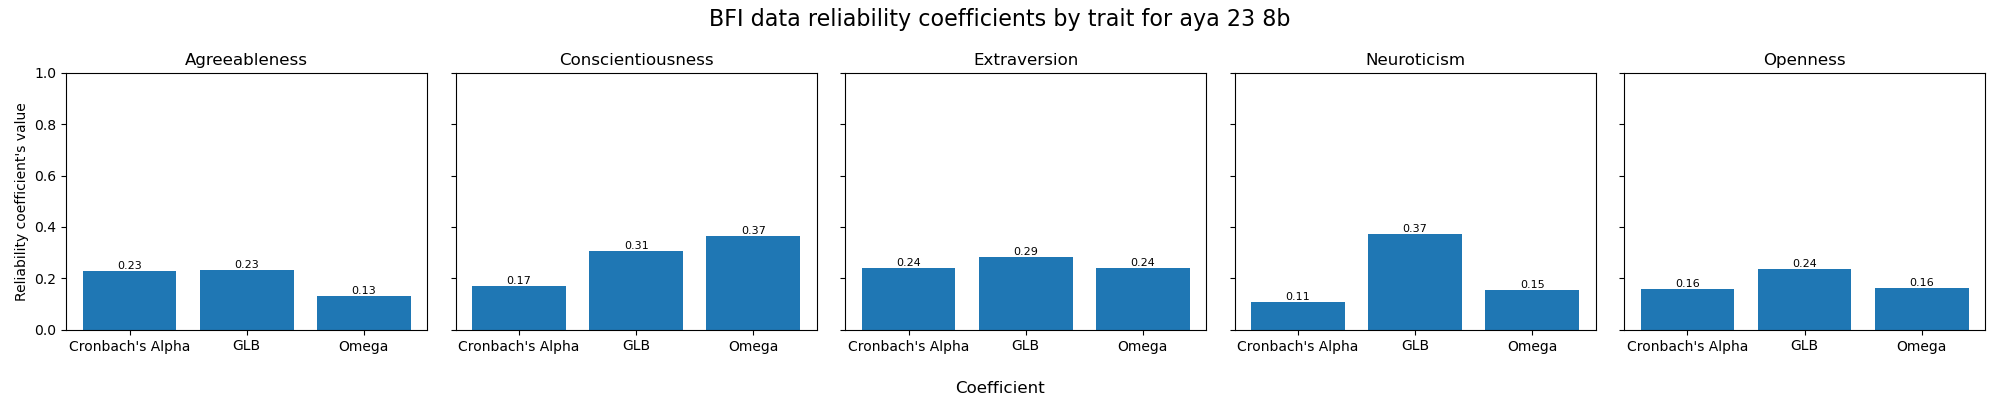
\includegraphics[width=0.7 \linewidth]{../Prompt_code/plots/aya-23-8b/bfi_reliability.png}
\end{figure}

\begin{figure}[H]
    \centering
    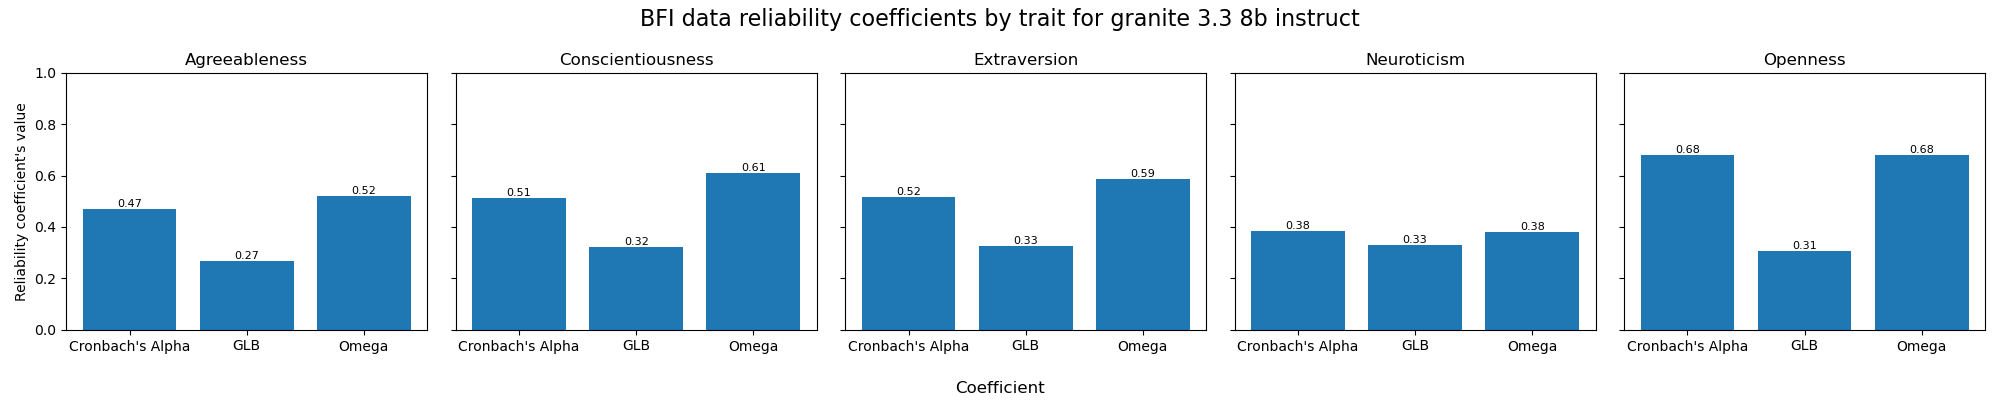
\includegraphics[width=0.7 \linewidth]{../Prompt_code/plots/granite-3.3-8b-instruct/bfi_reliability.png}
\end{figure}

\begin{figure}[H]
    \centering
    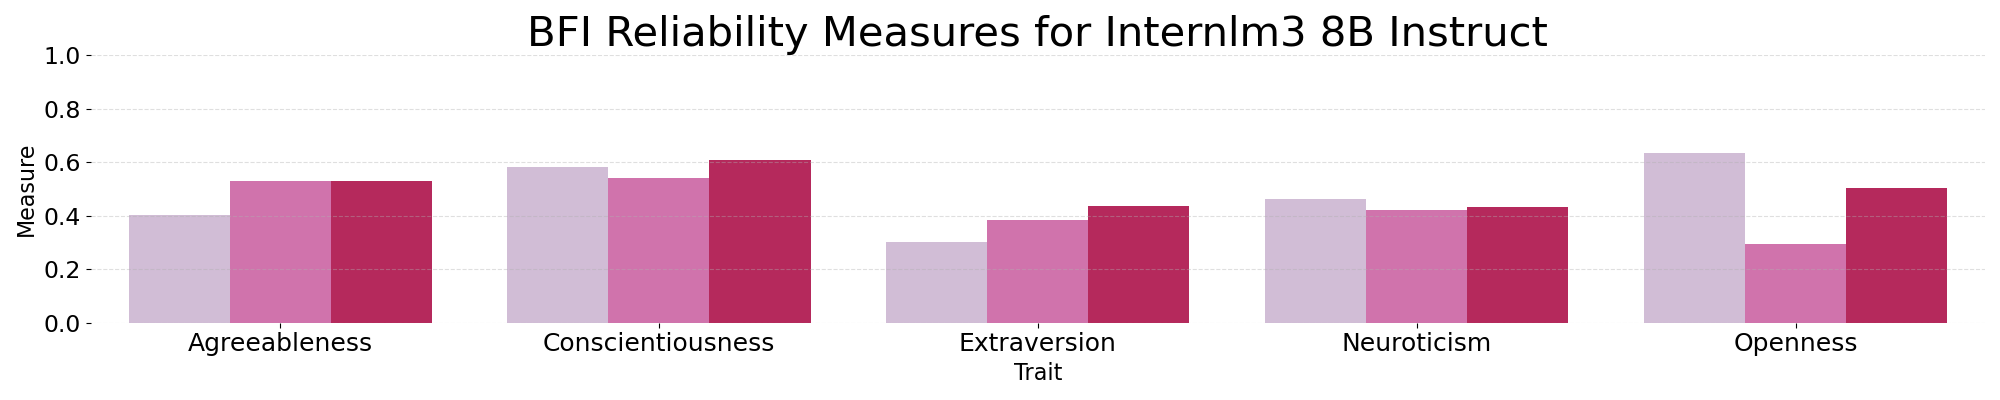
\includegraphics[width=0.7 \linewidth]{../Prompt_code/plots/internlm3-8b-instruct/bfi_reliability.png}
\end{figure}

\begin{figure}[H]
    \centering
    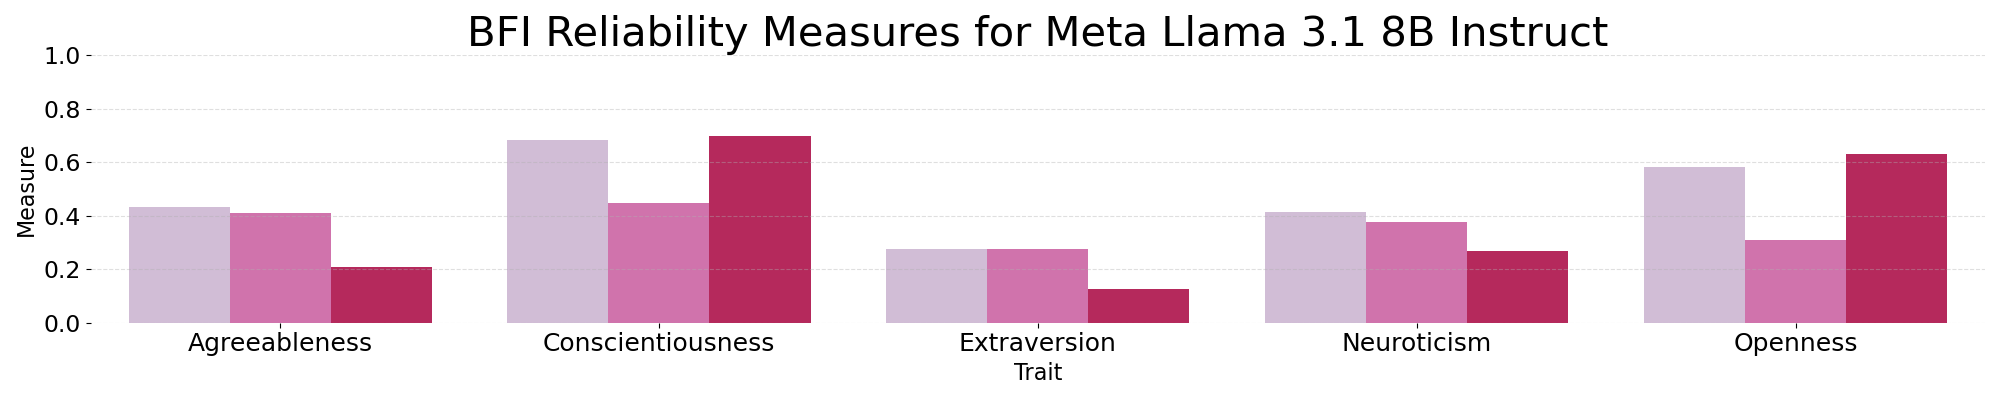
\includegraphics[width=0.7 \linewidth]{../Prompt_code/plots/meta-llama-3.1-8B-instruct/bfi_reliability.png}
\end{figure}

\begin{figure}[H]
    \centering
    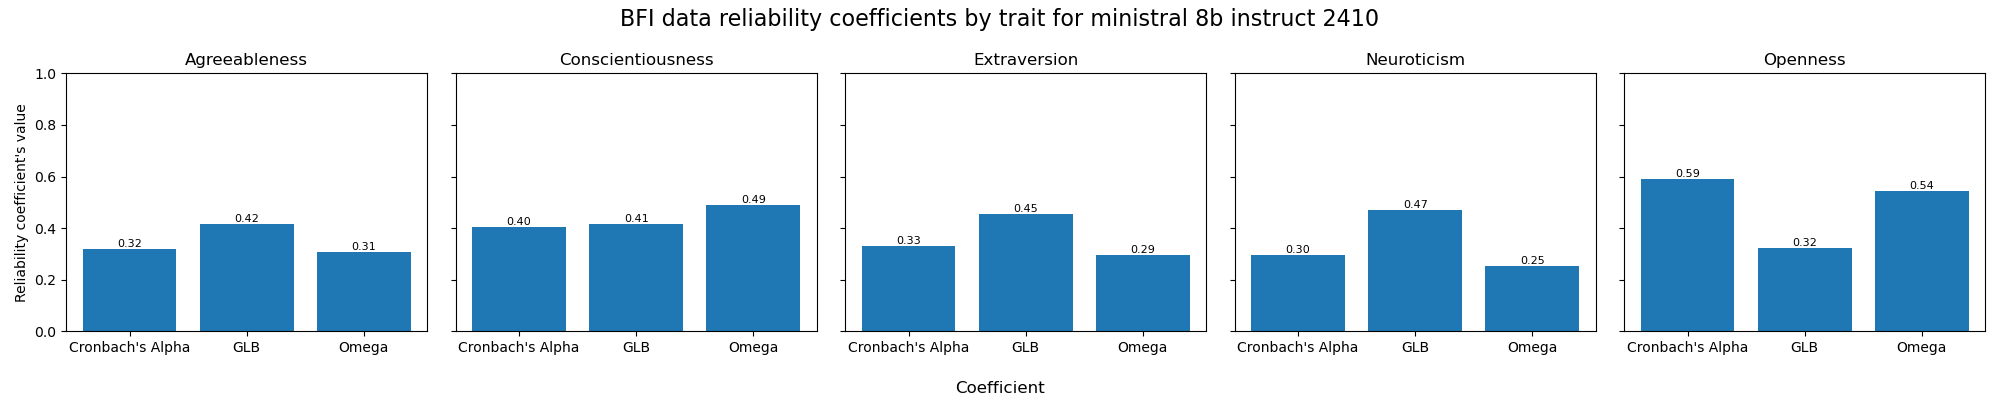
\includegraphics[width=0.7 \linewidth]{../Prompt_code/plots/ministral-8b-instruct-2410/bfi_reliability.png}
\end{figure}

\begin{figure}[H]
    \centering
    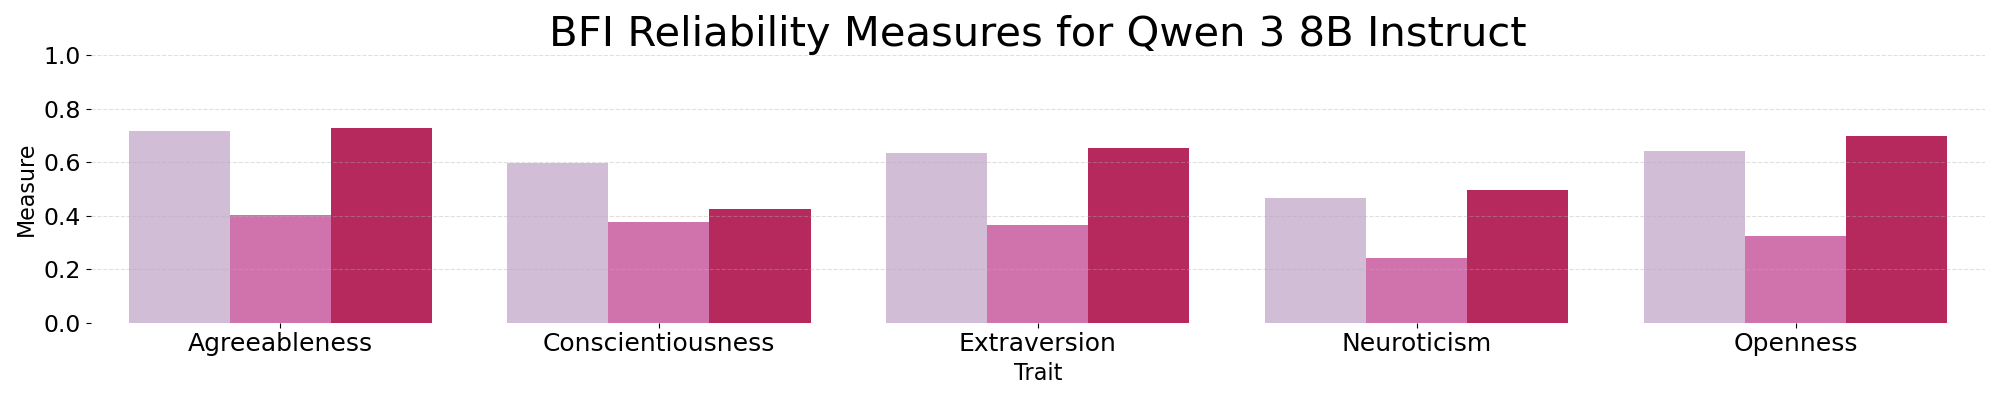
\includegraphics[width=0.7 \linewidth]{../Prompt_code/plots/qwen-3-8b-instruct/bfi_reliability.png}
\end{figure}

Wyniki w podanych miarach mogą nie napawać optymizmem. Tylko niektóre modele zbliżają się do granicy o wartości 0.7. Mając jednak na uwadze ograniczenie naszych modeli oraz skuteczność wykorzystanych kwestionariuszy, musimy stwierdzić winę w modelach. \\


Wyniki naszego eksperymentu będziemy porównywać z wynikami ludzkimi oraz modeli autorów przytaczanego artykułu, których wykresy są zaczerpnięte z artykułu. 
W wynikach skupimy się na BFI z uwagi na to, że był głównie wykorzystany w artykule i będziemy mieli oczywiste porównanie wyników obu eksperymentów.

Przeanalizujemy na początek dystrybucje odpowiedzi modeli dla poszczególnych kwestionariuszy i cech. Porównanie wyników modeli dla kwestionariusza BFI oraz ludzkich odpowiedzi przedstawia się następująco:

\begin{figure}[H]
    \centering
    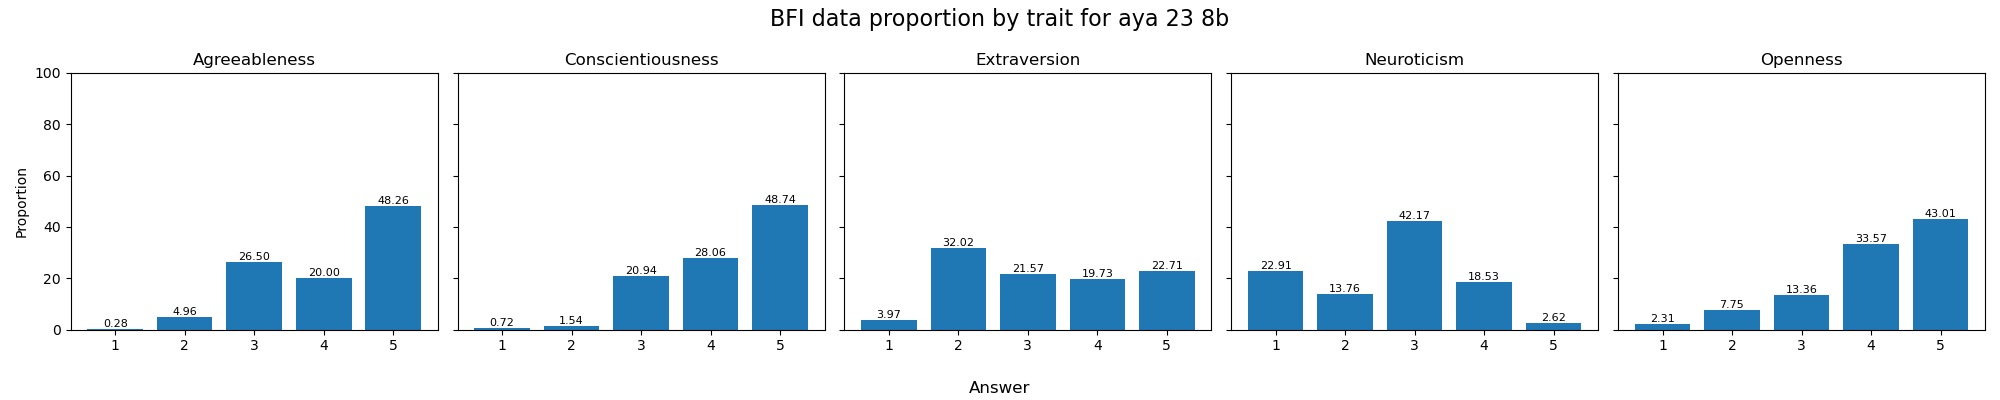
\includegraphics[width=0.7 \linewidth]{../Prompt_code/plots/aya-23-8b/bfi_distribution.png}
\end{figure}

\begin{figure}[H]
    \centering
    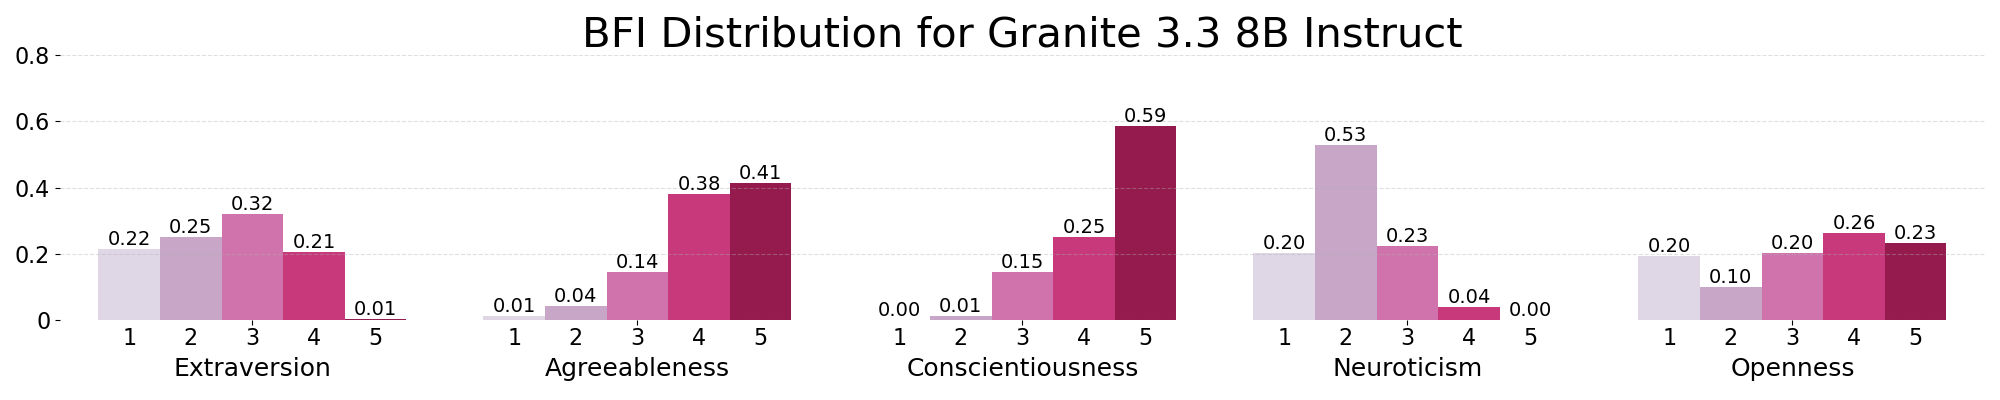
\includegraphics[width=0.7 \linewidth]{../Prompt_code/plots/granite-3.3-8b-instruct/bfi_distribution.png}
\end{figure}

\begin{figure}[H]
    \centering
    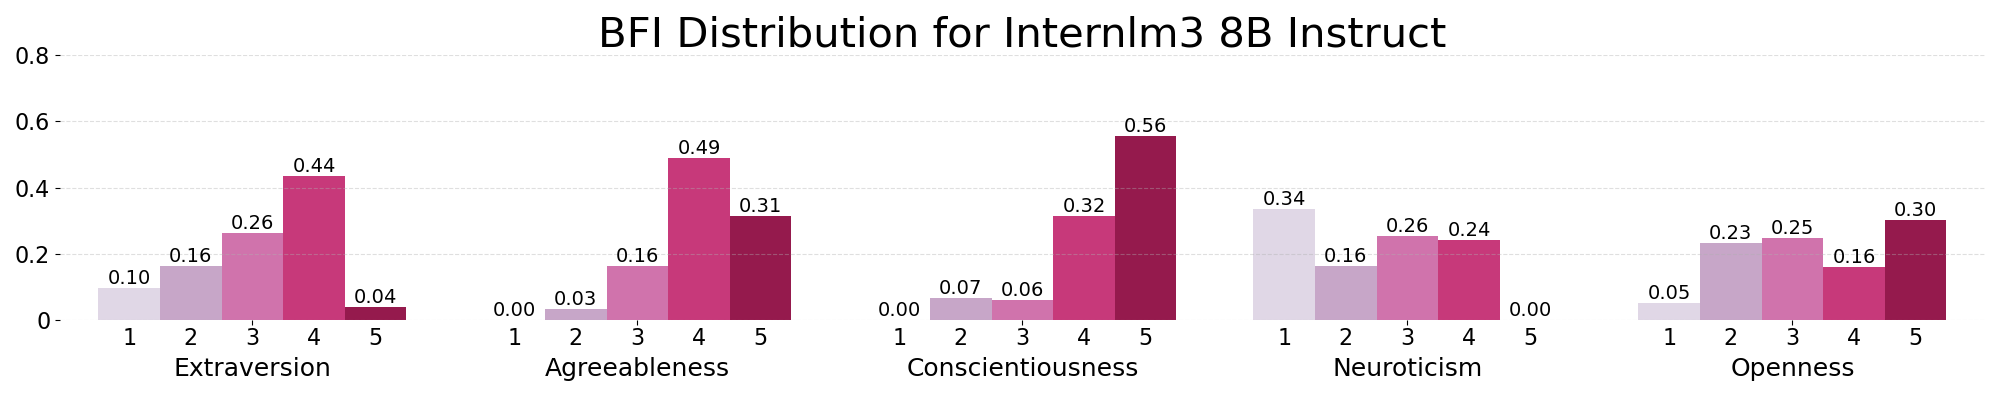
\includegraphics[width=0.7 \linewidth]{../Prompt_code/plots/internlm3-8b-instruct/bfi_distribution.png}
\end{figure}

\begin{figure}[H]
    \centering
    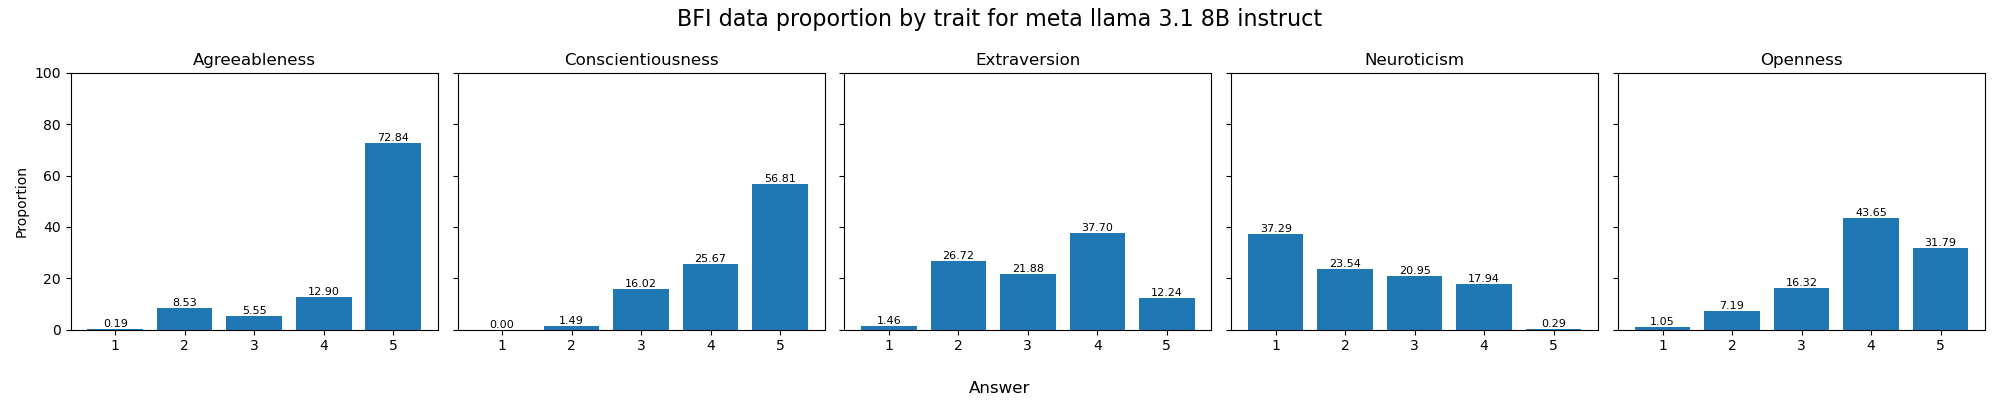
\includegraphics[width=0.7 \linewidth]{../Prompt_code/plots/meta-llama-3.1-8B-instruct/bfi_distribution.png}
\end{figure}

\begin{figure}[H]
    \centering
    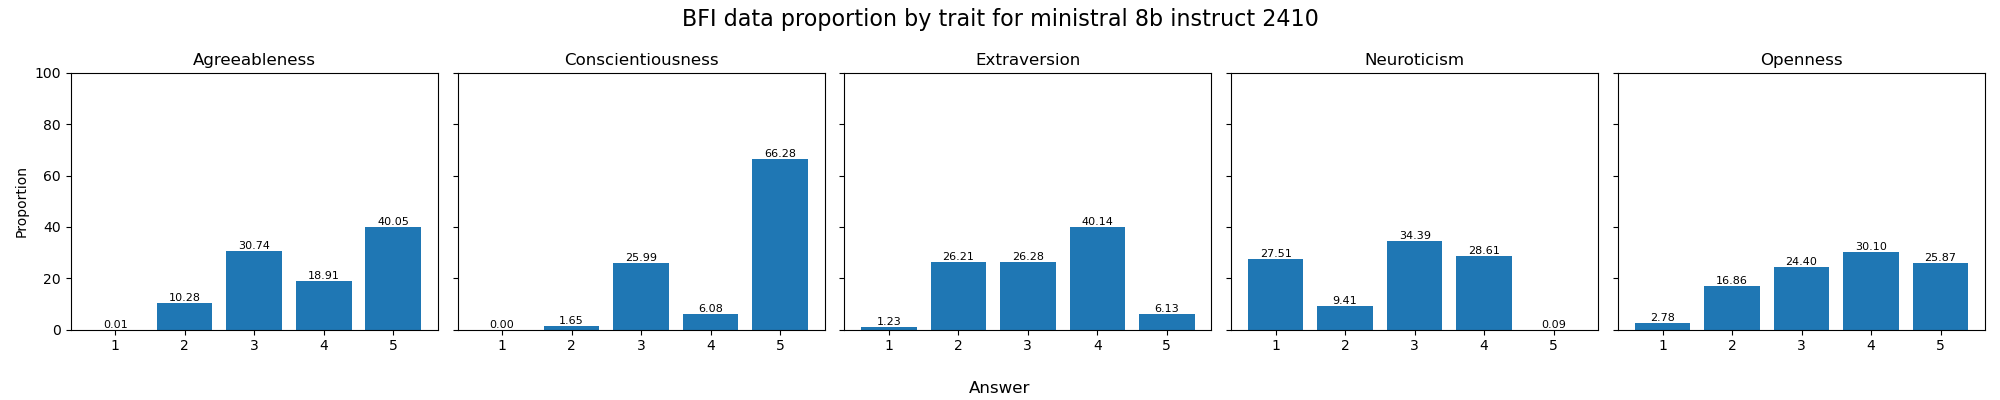
\includegraphics[width=0.7 \linewidth]{../Prompt_code/plots/ministral-8b-instruct-2410/bfi_distribution.png}
\end{figure}

\begin{figure}[H]
    \centering
    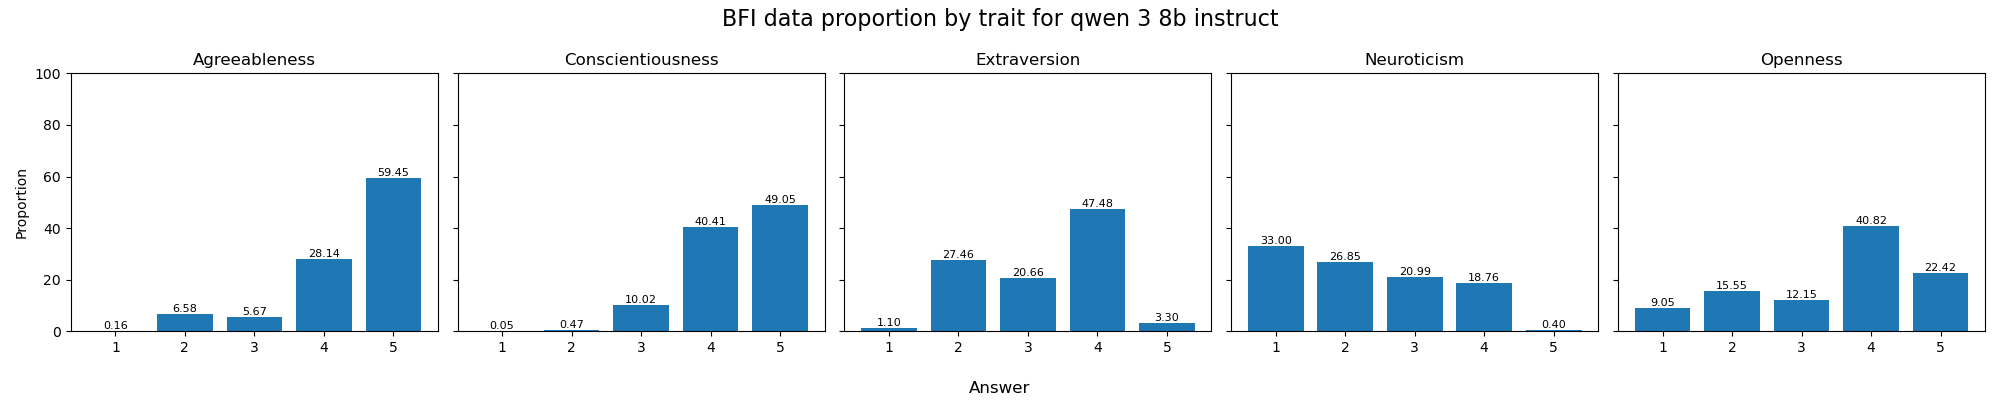
\includegraphics[width=0.7 \linewidth]{../Prompt_code/plots/qwen-3-8b-instruct/bfi_distribution.png}
\end{figure}

Wyniki ludzkie podane przez twórców artykułu:

\begin{figure}[H]
    \centering
    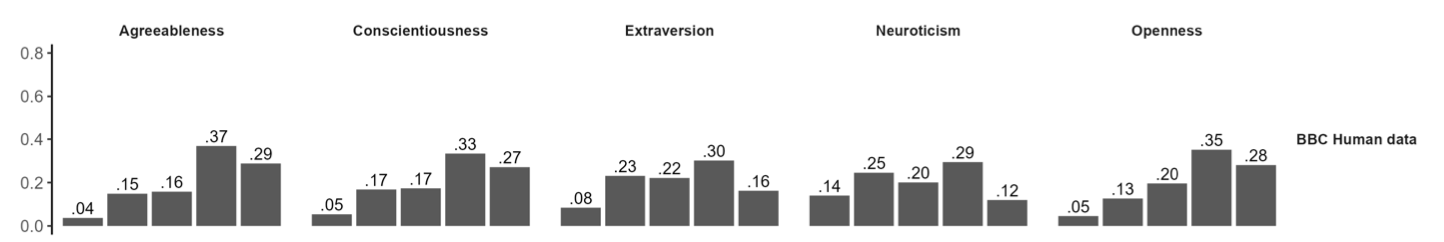
\includegraphics[width=0.7 \linewidth]{./article_data/human_distr.png}
\end{figure}

Zauważyć można różne dystrybucje w przypadku różnych modeli. Pare modeli ma podobną dystrybucje w tych samym atrybutach, jednak brak takich, które w każdym atrybucie miałyby taki sam rozkład odpowiedzi. \\
W przypadku Agreeableness modele w większości odpowiadały 5, wyjątkiem jest InternLM, który najczęściej odpowiada 4. \\
Dla Conscientiousness wszsytkie modele odpowiadały podobnie, poza Ministral, który nie udzielał odpowiedzi 4. \\
Dystrybucja Extraversion dystrubucja jest stosunkowo wyrównania po środku w odpowiedziach 2, 3 i 4. \\
W Neuroticism odpowiedzi są średnio niższe, praktycznie bez 5. \\
Openenness nie ma stałej struktury, modele poróżniły się dla tej cechy. \\
Porównując z odpowiedziami ludzi, ciężko o pełne podobieństwo i w przeważającej większości dystrybucje różnią się.  Jednak dla pojedyńczych dystrybucji jest bardzo duże podobnieństwo.\\ \\ 

Kolejną ważną kwestią jest porównianie korelacji odpowiedzi dla atrybutów na tle korelacji w odpowiedziach ludzi. Pokaże to, czy modele są wyuczone zależności, które nie występują w rzeczywistości.

\begin{figure}[H]
    \centering
    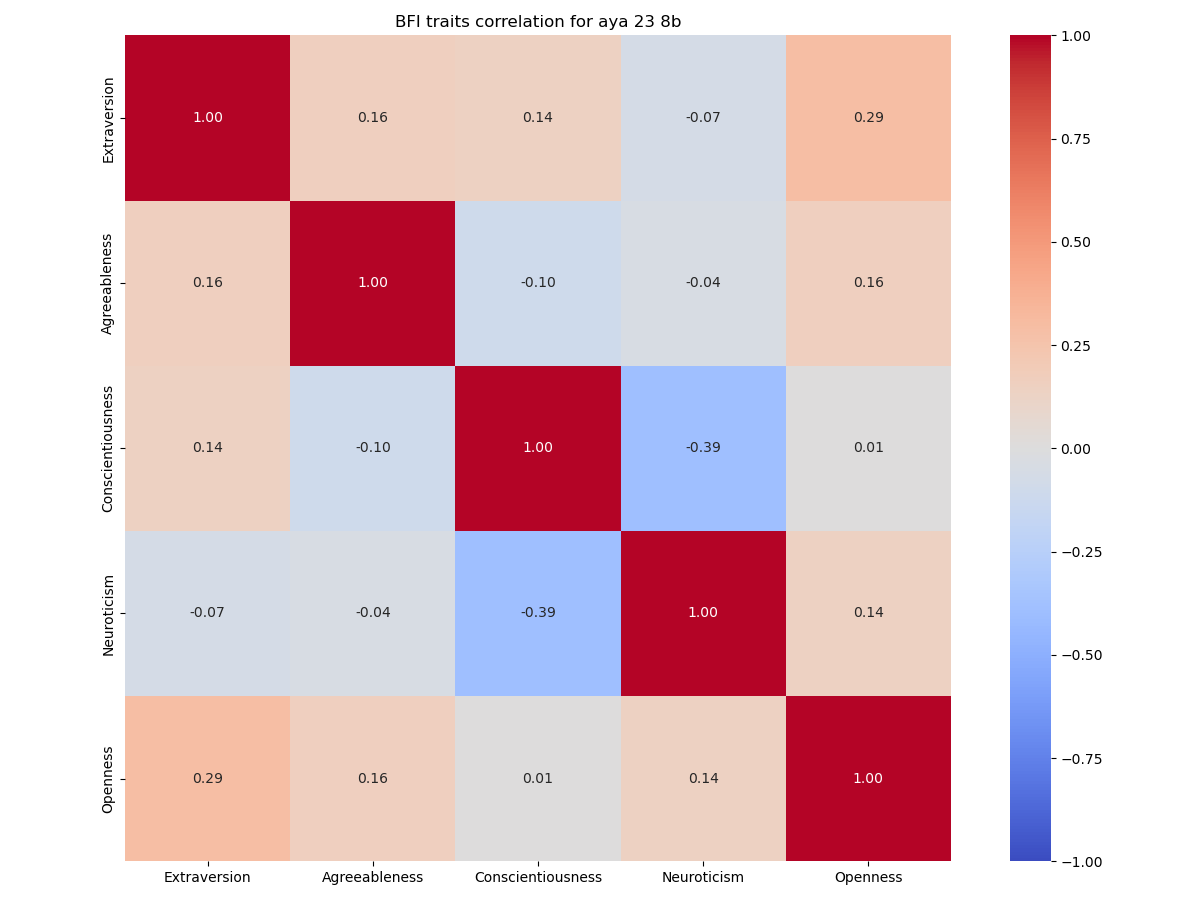
\includegraphics[width=0.7 \linewidth]{../Prompt_code/plots/aya-23-8b/bfi_correlation.png}
\end{figure}

\begin{figure}[H]
    \centering
    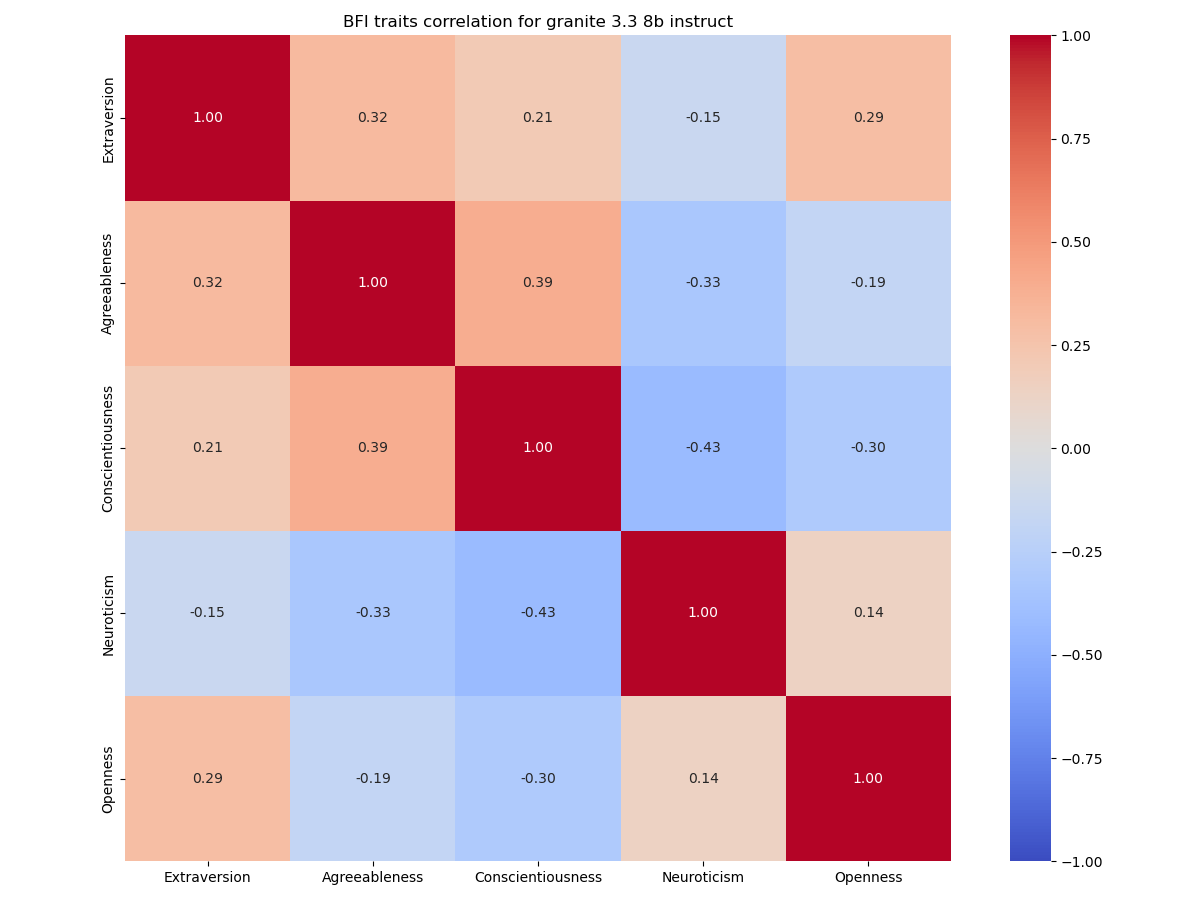
\includegraphics[width=0.7 \linewidth]{../Prompt_code/plots/granite-3.3-8b-instruct/bfi_correlation.png}
\end{figure}

\begin{figure}[H]
    \centering
    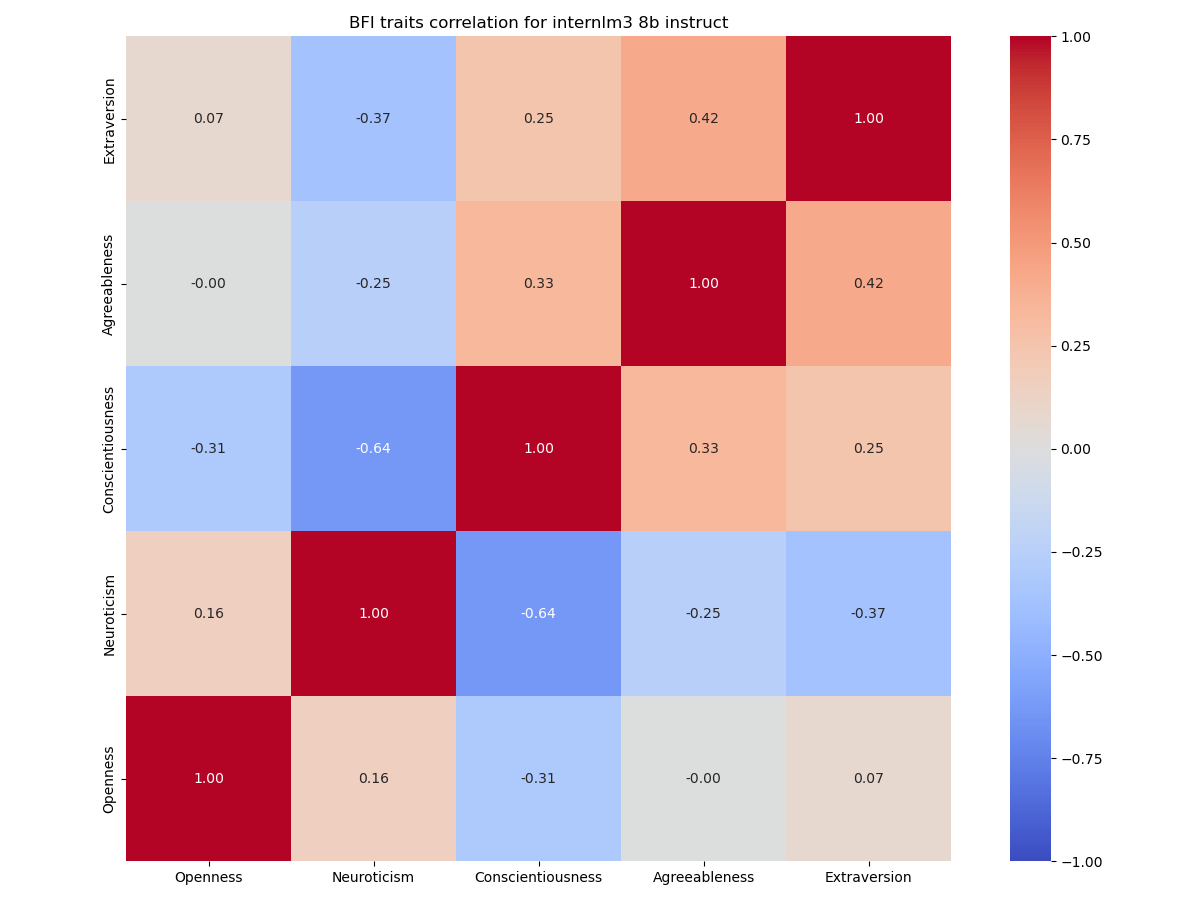
\includegraphics[width=0.7 \linewidth]{../Prompt_code/plots/internlm3-8b-instruct/bfi_correlation.png}
\end{figure}

\begin{figure}[H]
    \centering
    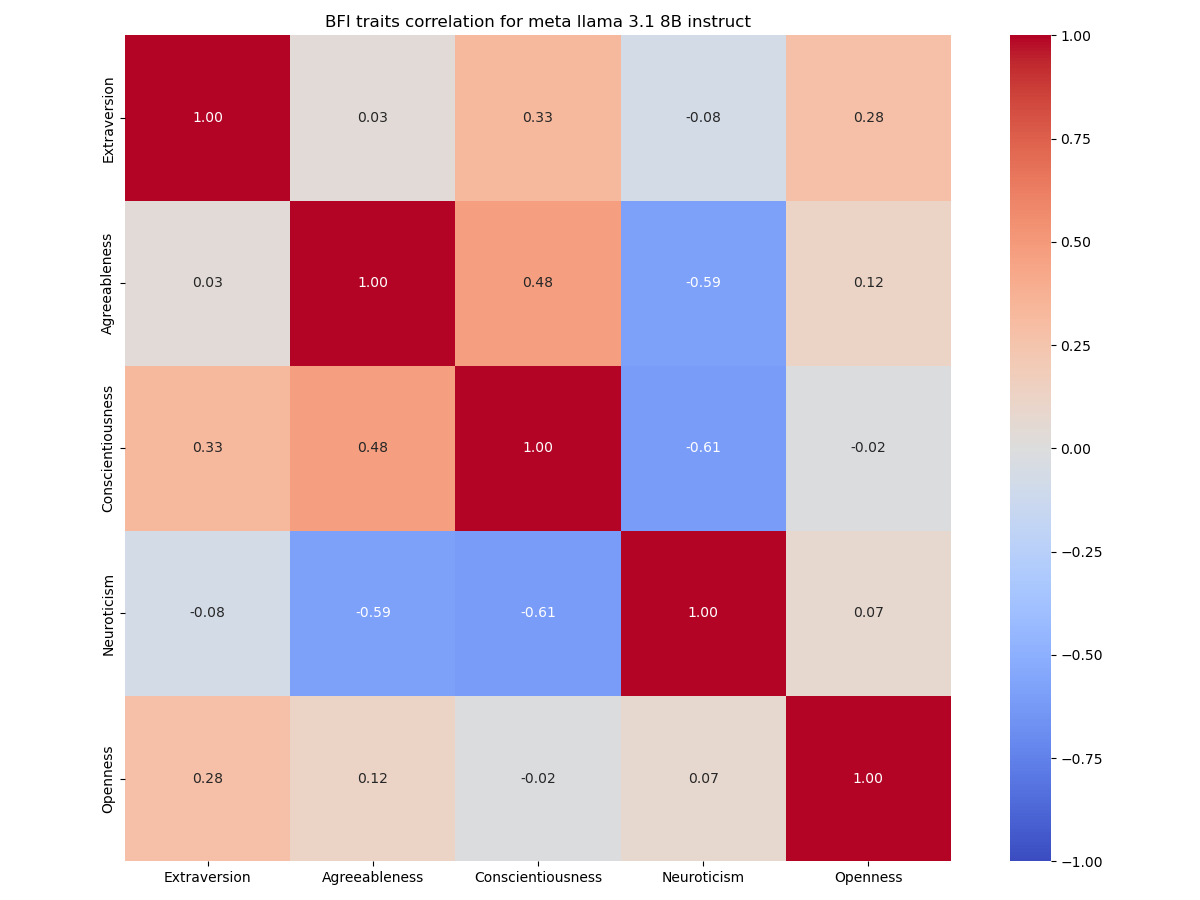
\includegraphics[width=0.7 \linewidth]{../Prompt_code/plots/meta-llama-3.1-8B-instruct/bfi_correlation.png}
\end{figure}

\begin{figure}[H]
    \centering
    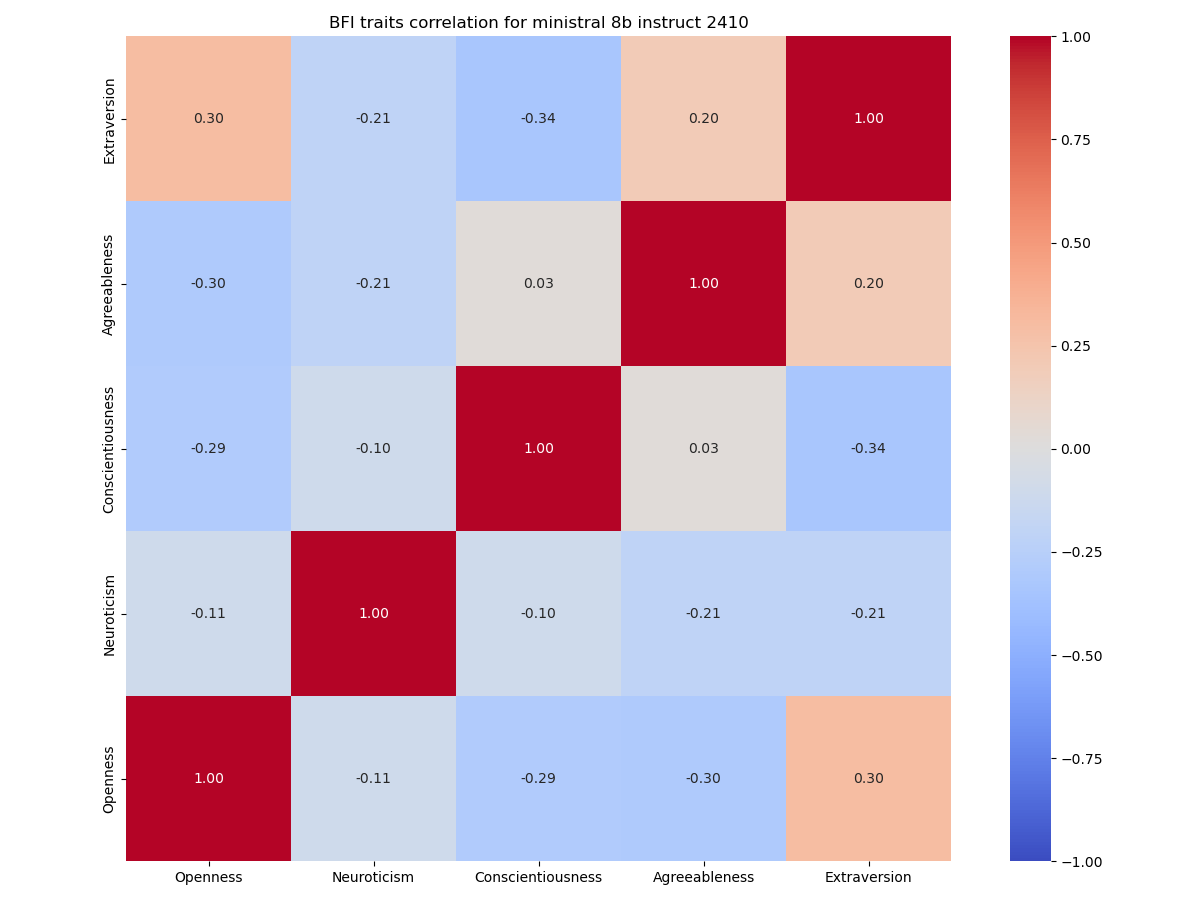
\includegraphics[width=0.7 \linewidth]{../Prompt_code/plots/ministral-8b-instruct-2410/bfi_correlation.png}
\end{figure}

\begin{figure}[H]
    \centering
    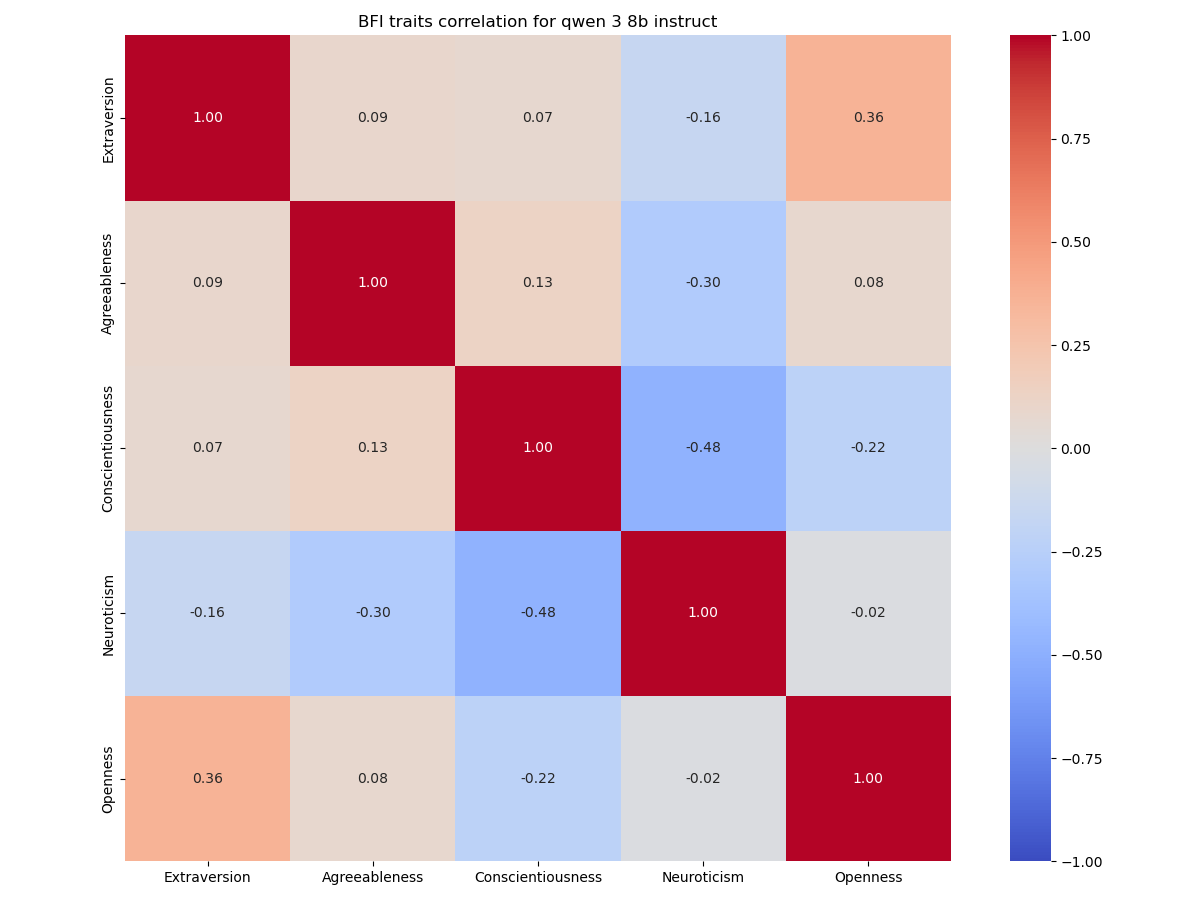
\includegraphics[width=0.7 \linewidth]{../Prompt_code/plots/qwen-3-8b-instruct/bfi_correlation.png}
\end{figure}

\begin{figure}[H]
    \centering
    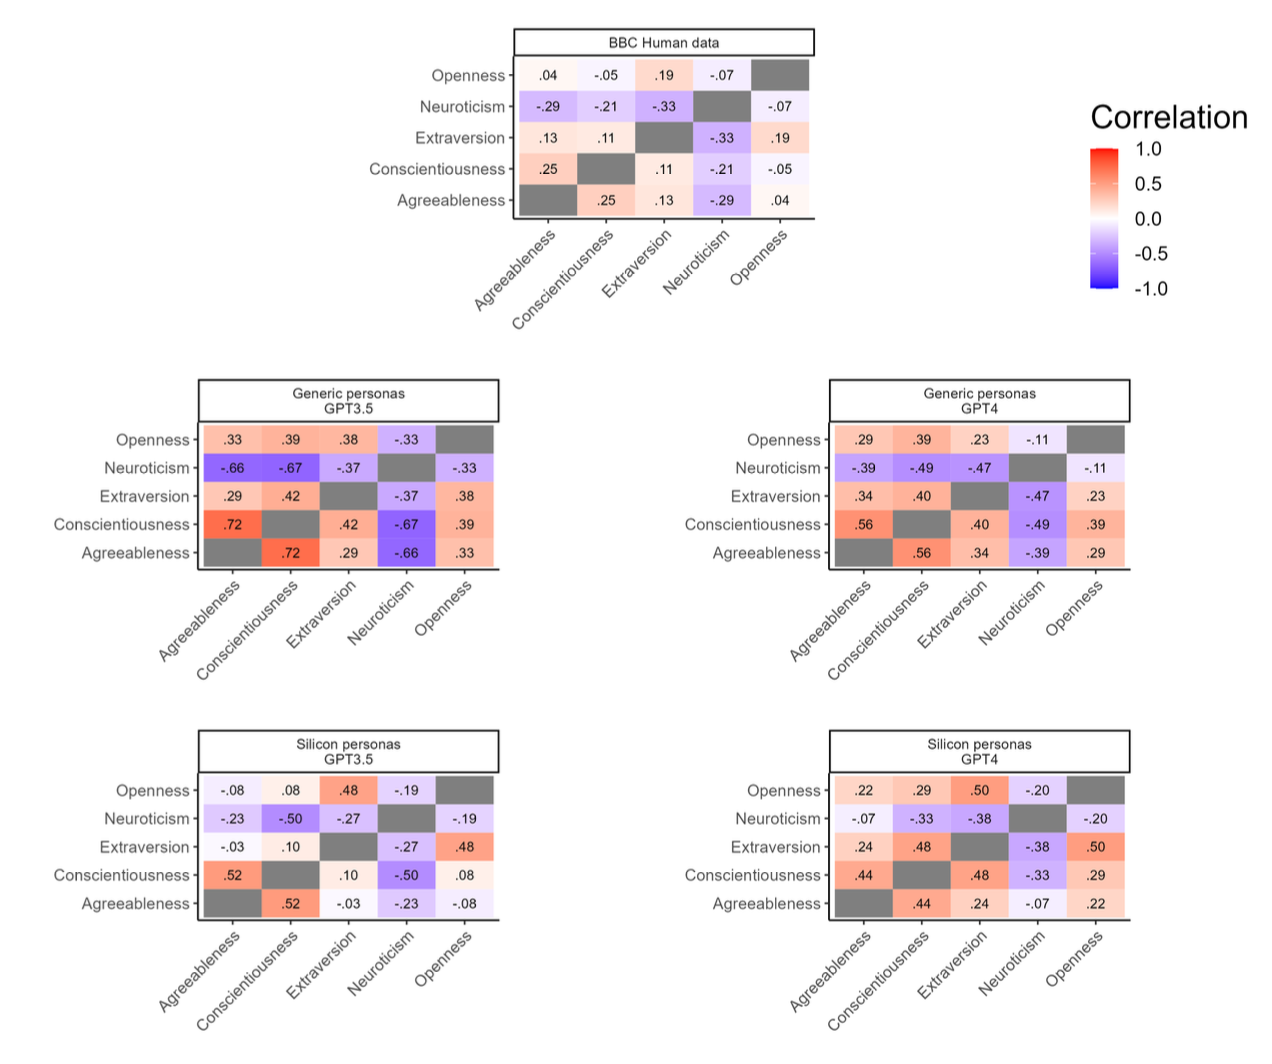
\includegraphics[width=0.7 \linewidth]{./article_data/all_corr.png}
\end{figure}

Dla Neuroticism korelacje wyników modeli przypominają te ludzkie. Reszta korelacji nie przekracza w wartości bezwzględnej 0.4. Jednak patrząc ogólnie wartości są wyższe niż dla wyników ludzkich, co pokrywa się z wynikami otrzymanami przez autorów przytaczanego artykułu, chociaż u nich wartości były dodatnie.

Poniżej przedstawiono analizę Korelacji Pearsona pomiędzy kwestionariusza.
\newpage
\begin{figure}[H]
    \centering
    \begin{subfigure}{0.38\textwidth}
        \centering
        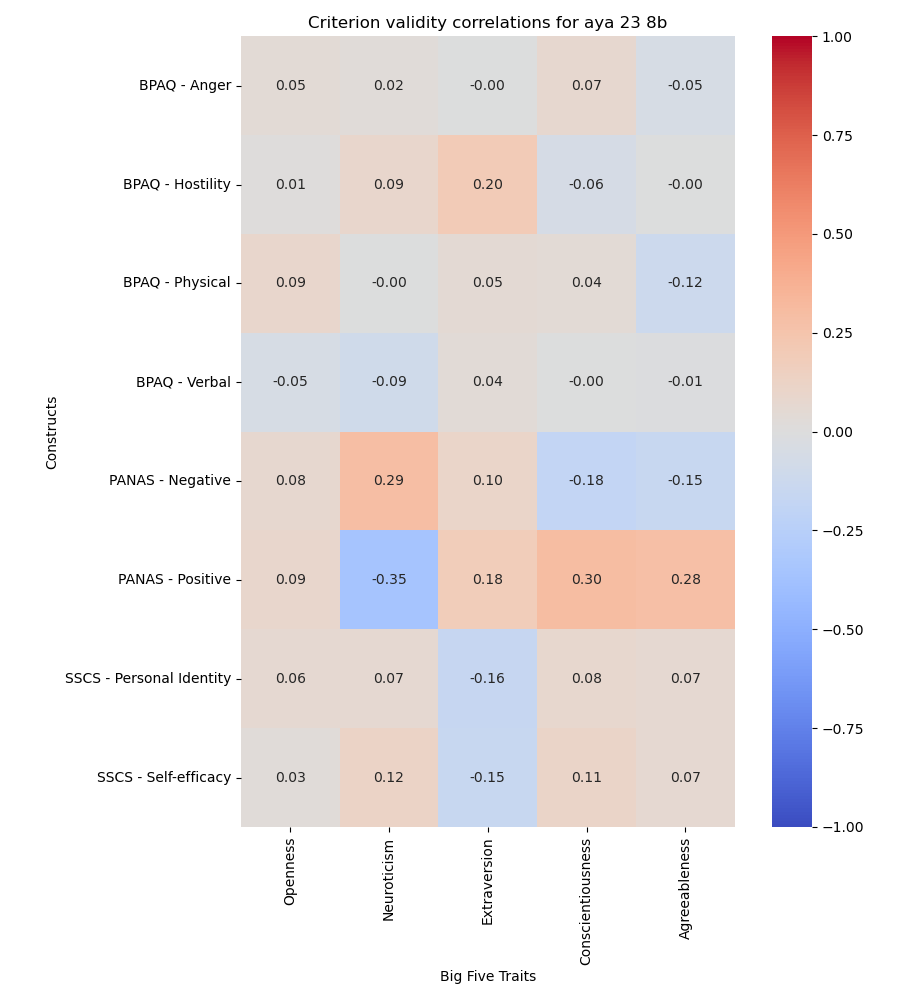
\includegraphics[width=\linewidth]{../Prompt_code/plots/aya-23-8b/crit_val_correlation.png}
    \end{subfigure}
    \begin{subfigure}{0.38\textwidth}
        \centering
        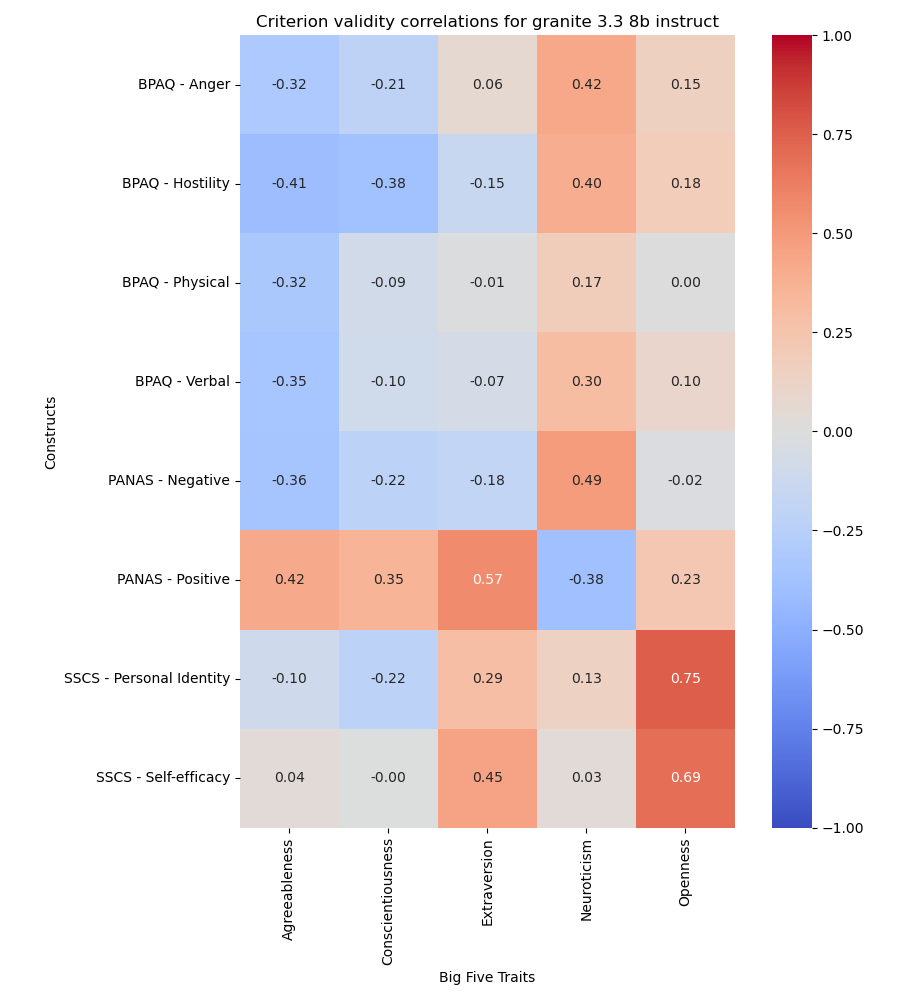
\includegraphics[width=\linewidth]{../Prompt_code/plots/granite-3.3-8b-instruct/crit_val_correlation.png}
    \end{subfigure}
\end{figure}

\begin{figure}[H]
    \centering
    \begin{subfigure}{0.38\textwidth}
        \centering
        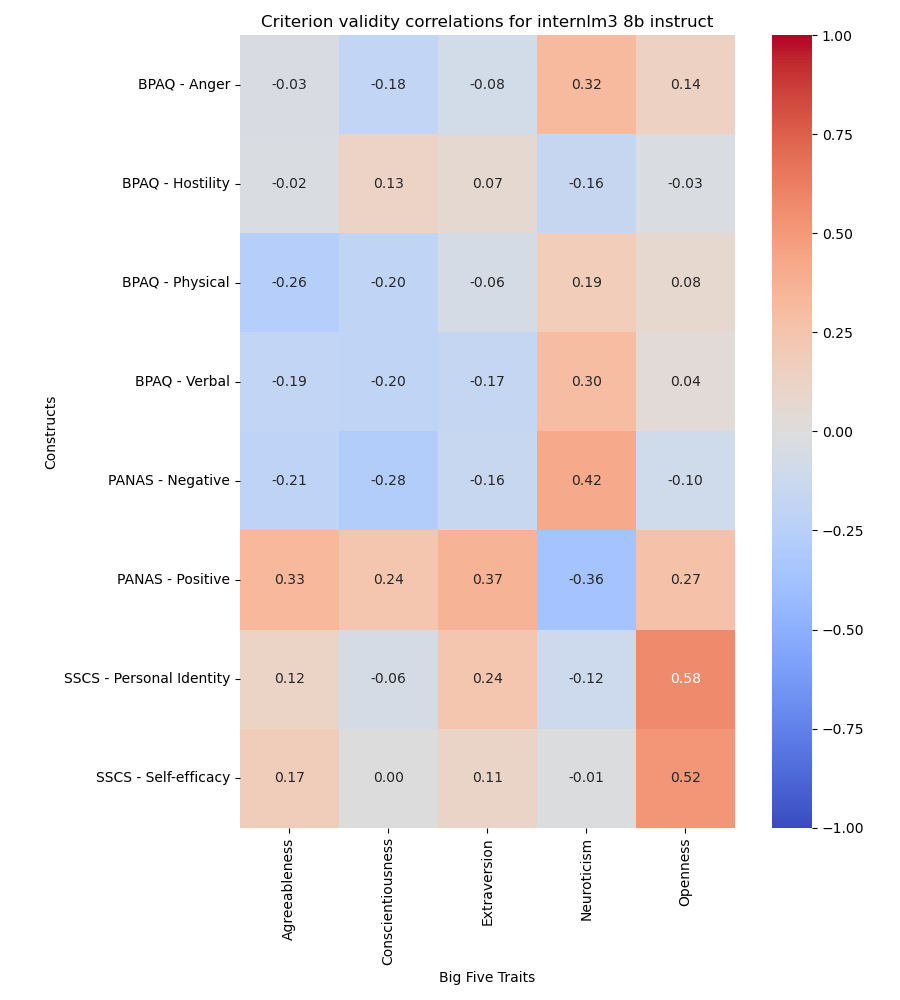
\includegraphics[width=\linewidth]{../Prompt_code/plots/internlm3-8b-instruct/crit_val_correlation.png}
    \end{subfigure}
    \begin{subfigure}{0.38\textwidth}
        \centering
        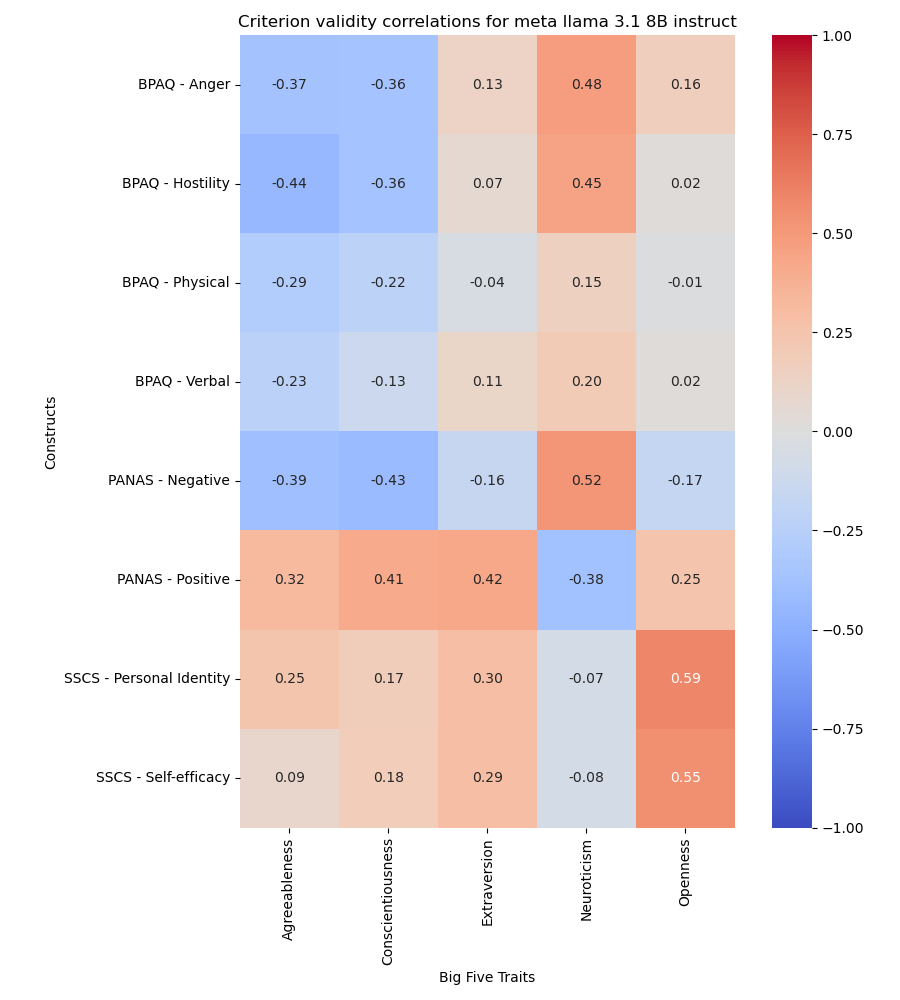
\includegraphics[width=\linewidth]{../Prompt_code/plots/meta-llama-3.1-8B-instruct/crit_val_correlation.png}
    \end{subfigure}
\end{figure}

\begin{figure}[H]
    \centering
    \begin{subfigure}{0.38\textwidth}
        \centering
        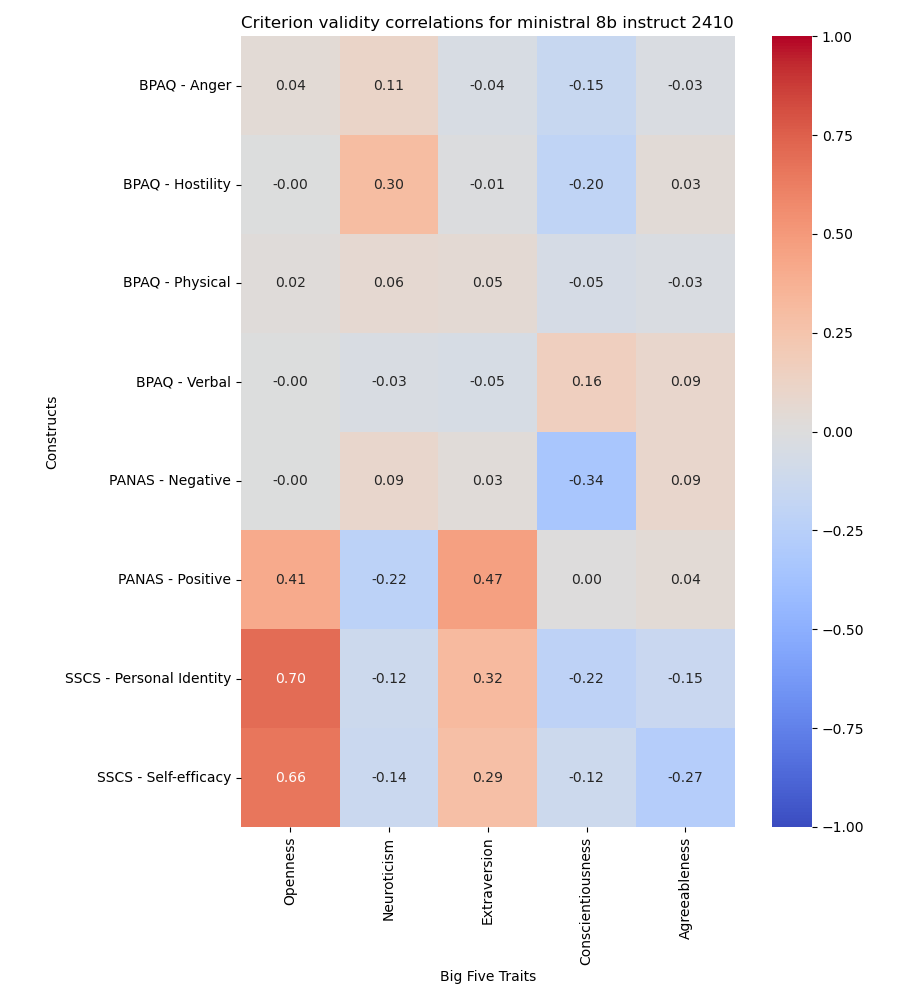
\includegraphics[width=\linewidth]{../Prompt_code/plots/ministral-8b-instruct-2410/crit_val_correlation.png}
    \end{subfigure}
    \begin{subfigure}{0.38\textwidth}
        \centering
        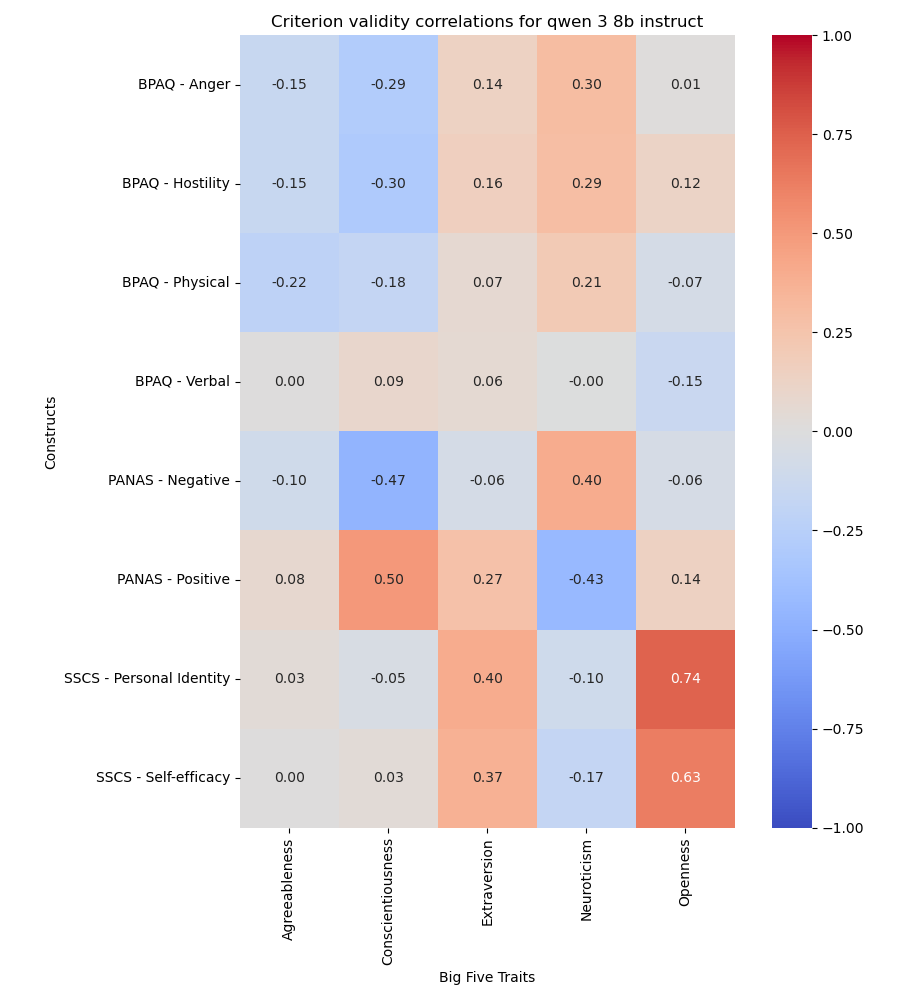
\includegraphics[width=\linewidth]{../Prompt_code/plots/qwen-3-8b-instruct/crit_val_correlation.png}
    \end{subfigure}
\end{figure}

\newpage
Wyniki autorów.

\begin{figure}[H]
    \centering
    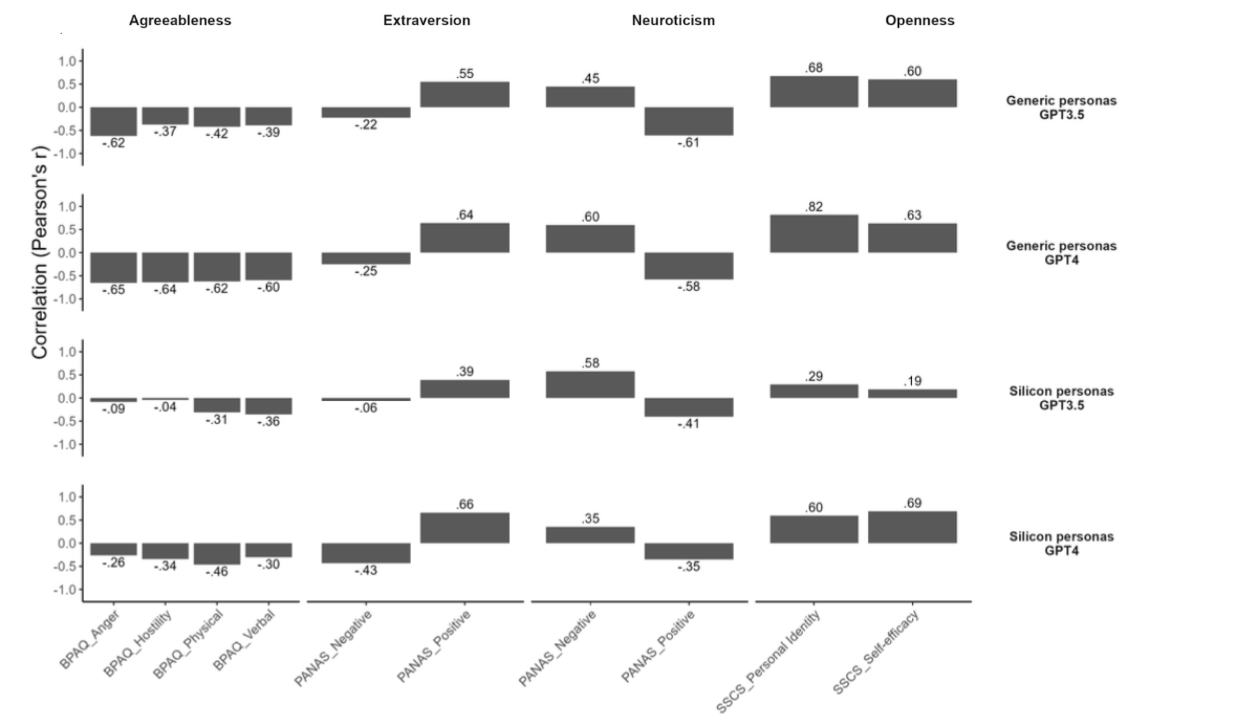
\includegraphics[width=0.7 \linewidth]{./article_data/cross_corr.png}
\end{figure}

Wartości korelacji mają wartości bezwzględne poniżej 0.4, pomijając kwestionariusz SSCS, dla które zaobserowano wysokie wyniki. \\
Wysokie wyniki dla SSCS pokrywają się z poprzenimi badaniami. Dla innych kwestionariuszy wartości są bliższe zeru, co jest znaczącą różnicą.

\section{Wnioski}
Jakość odpowiedzi może budzić niepokój z uwagi na wartości miar walidujących jakość testów. Mając jednak świadomość niezawodności kwestionariuszy, musimy stwierdzić winę w odpowiedziach modeli. \\
Odpowiedzi modeli różnią się od tych ludzkich pod względem dystrybucji, co pokazuję ich słabość w odzworowywaniu ludzkich odpowiedzi. Występują korelacje między cechami poza cechą neurotyzmu, co nie zgadza się z prawdziwymi wynikami. \\
Na podstawie otrzymanych wynik możemy stwierdzić niezdolność LLM do symulowania ludzkich zachowań psychologicznych. Obecnie modele nie nadają się do symulowania i pomimo zmiany opisów osób nie osiągnięto lepszych rezultatów. Potwierdza to naszą tezę. \\
Analizując wyniki poszczególnych modeli, zauważyć można różnice zarówno w dystrybucji jak i korelacjach odpowiedzi. Wnioskujemy z tego, że pochodzenie modelu wpływa na ich wyniki w testach psychologicznych. Zgadza się to z naszą tezą.

\section{Future works}
W najbliższych tygodniach planowane jest zwiększenie liczby zgromadzonych odpowiedzi oraz rozszerzenie danych wejściowych o elementy interakcji między personami, realizowane w formie dialogów. 
Taki zabieg mógłby wprowadzić dodatkową warstwę emocjonalną oraz złożoność psychospołeczną do opisów, co potencjalnie wpłynęłoby na bardziej realistyczne i wielowymiarowe zachowania generowane przez modele.\\
Proces dalszej pracy, będzie podzielony tak jak poprzednio: Hubert Sobociński - promptowanie i przygotowanie danych z wyników, Paweł Pozorski - analiza wyników, Paweł Florek - przygotowanie wizualizacji i raportu.

W ramach dalszych badań proponujemy wykorzystanie bardziej zaawansowanych modeli językowych dostępnych na rynku oraz zastosowanie wydajniejszego sprzętu obliczeniowego. Pozwoli to na poprawę jakości generowanych odpowiedzi oraz znaczące skrócenie czasu ich pozyskiwania, co z kolei umożliwi zwiększenie wielkości próby badawczej.

\end{document}
